
\documentclass{beamer}
\usepackage[latin1]{inputenc}
%\usetheme{Montpellier}
%\usetheme{Boadilla}
%\usecolortheme[RGB={204,51,255}]{structure}
%\usecolortheme[named=purple]{structure}
\usecolortheme[RGB={62,128,62}]{structure}
%\definecolor{dark}{rgb}{0.3,0.15,0.3}
%\definecolor{light}{rgb}{0.8,0.6,0.8}
%\definecolor{reddish}{rgb}{.5,0.15,0.15}
\definecolor{dark}{rgb}{0.5,0.3,0.4}
%\definecolor{light}{rgb}{0.8,0.6,0.8}
\definecolor{reddish}{rgb}{.7,0.25,0.25}
\definecolor{greenish}{rgb}{.25,0.7,0.25}
\definecolor{blueish}{rgb}{.25,0.25,0.7}
\definecolor{purple}{rgb}{.5,0.0,0.5}
\usepackage{graphicx}
\usepackage{pstricks}

\setbeamertemplate{navigation symbols}{}

\newcommand{\crish}{\color{reddish}}
\newcommand{\cbla}{\color{black}}
\newcommand{\cred}{\color{red}}
\newcommand{\cblu}{\color{blue}}
\newcommand{\cgre}{\color{green}}

\newcommand{\sm}{\color{reddish}$}
\newcommand{\fm}{$\color{black}{}}

\newcommand{\letter}[1]{\color{blue}\texttt{#1}\color{black}}
\newcommand{\binary}[1]{\color{red}\texttt{#1}\color{black}}

\usepackage{tikz}
\usetikzlibrary{arrows,decorations.markings,positioning}
\usepackage{epstopdf}
\usetikzlibrary{fit}

\title[Information Theory lecture 5]{The data processing inequality: lecture 5}
\author{COMSM0075 Information Processing and Brain}
\institute{\texttt{comsm0075.github.io}}
\date{September 2020}

\begin{document}

\maketitle

\begin{frame}{Snakes and Ladders or Moksha Patam}
  \begin{center}
    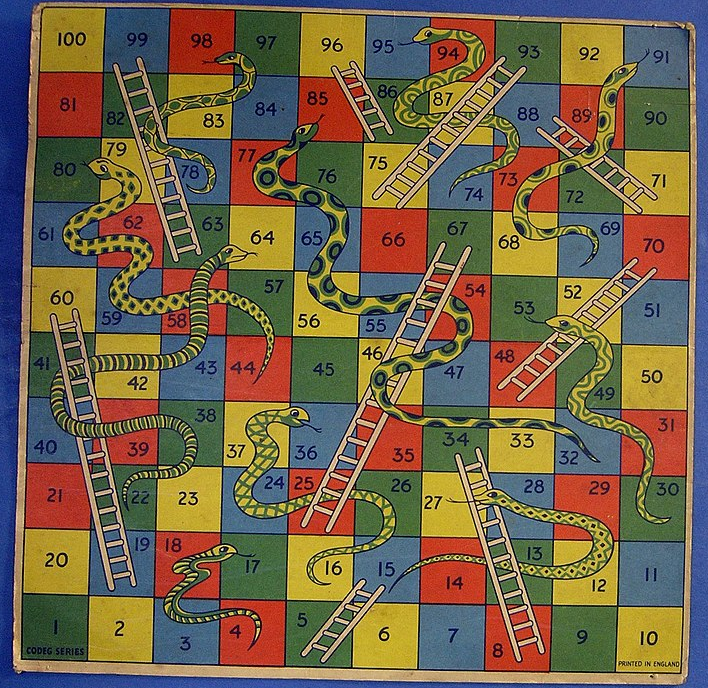
\includegraphics[width=8cm]{game.png}
  \end{center}
    \vfill
\tiny{\flushright{Image from wikipedia.}}
\end{frame}


\begin{frame}{start at 1}
  \begin{center}
    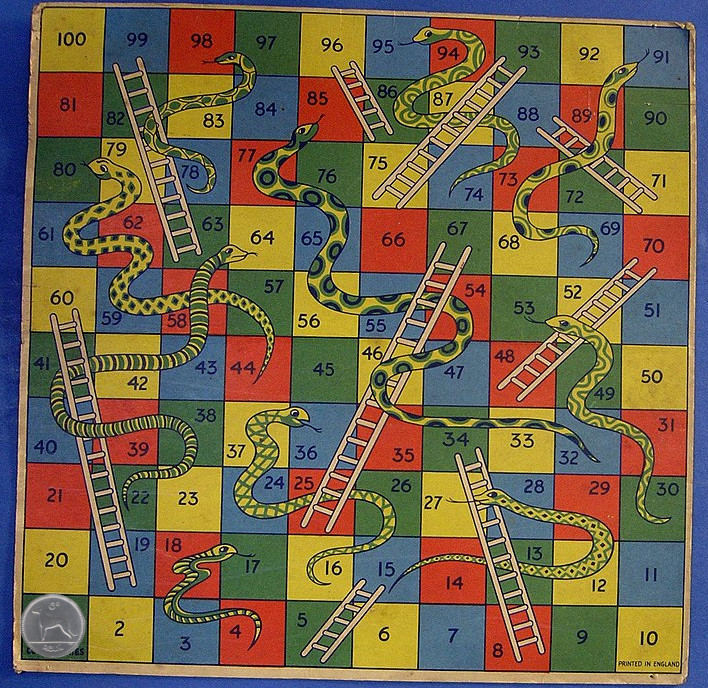
\includegraphics[width=8cm]{game1.jpg}
  \end{center}
    \vfill
\tiny{\flushright{Image from wikipedia.}}
\end{frame}


\begin{frame}{1$\rightarrow$5 (roll 4)}
  \begin{center}
    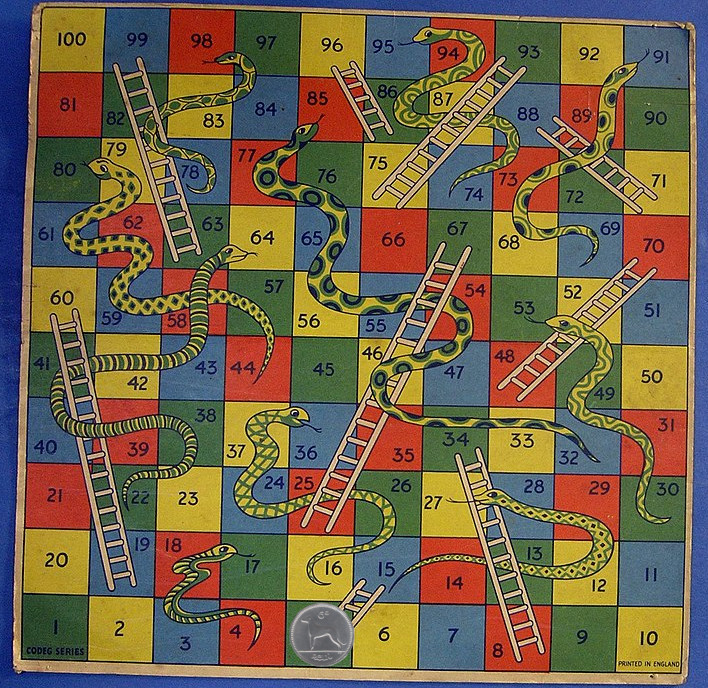
\includegraphics[width=8cm]{game5.jpg}
  \end{center}
    \vfill
\tiny{\flushright{Image from wikipedia.}}
\end{frame}


\begin{frame}{1$\rightarrow$15 (up the ladder)}
  \begin{center}
    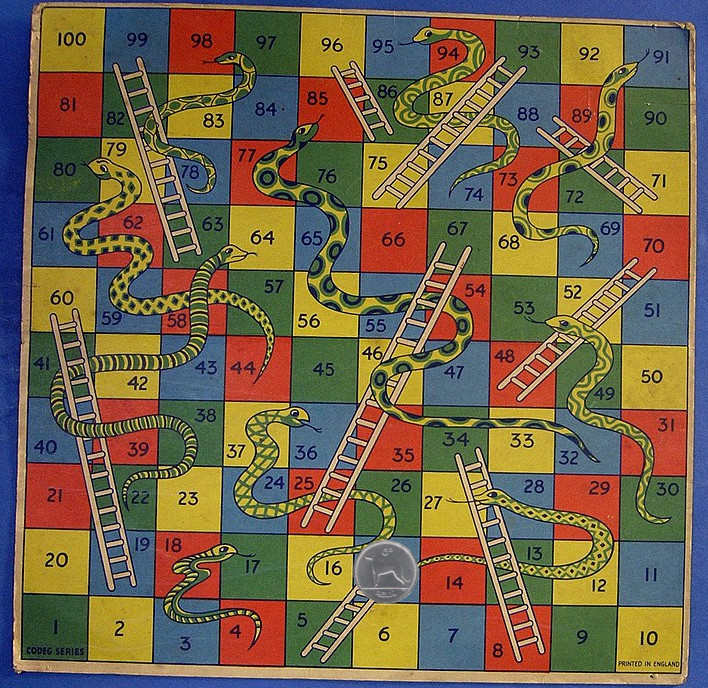
\includegraphics[width=8cm]{game15.jpg}
  \end{center}
    \vfill
\tiny{\flushright{Image from wikipedia.}}
\end{frame}


\begin{frame}{1$\rightarrow$15$\rightarrow$19 (roll another 4)}
  \begin{center}
    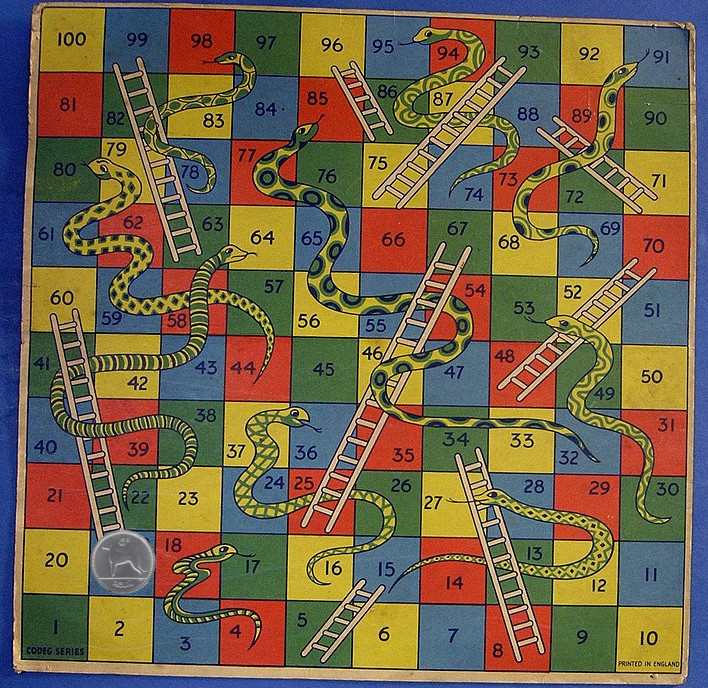
\includegraphics[width=8cm]{game19.jpg}
  \end{center}
    \vfill
\tiny{\flushright{Image from wikipedia.}}
\end{frame}


\begin{frame}{1$\rightarrow$15$\rightarrow$19$\rightarrow$60 (up the ladder)}
  \begin{center}
    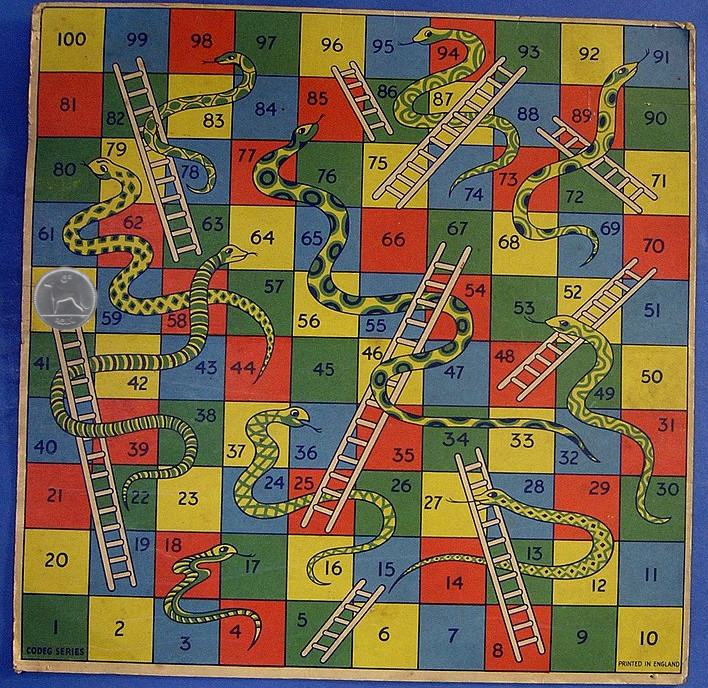
\includegraphics[width=8cm]{game60.jpg}
  \end{center}
    \vfill
\tiny{\flushright{Image from wikipedia.}}
\end{frame}


\begin{frame}{1$\rightarrow$15$\rightarrow$19$\rightarrow$60$\rightarrow$63 (roll a 3)}
  \begin{center}
    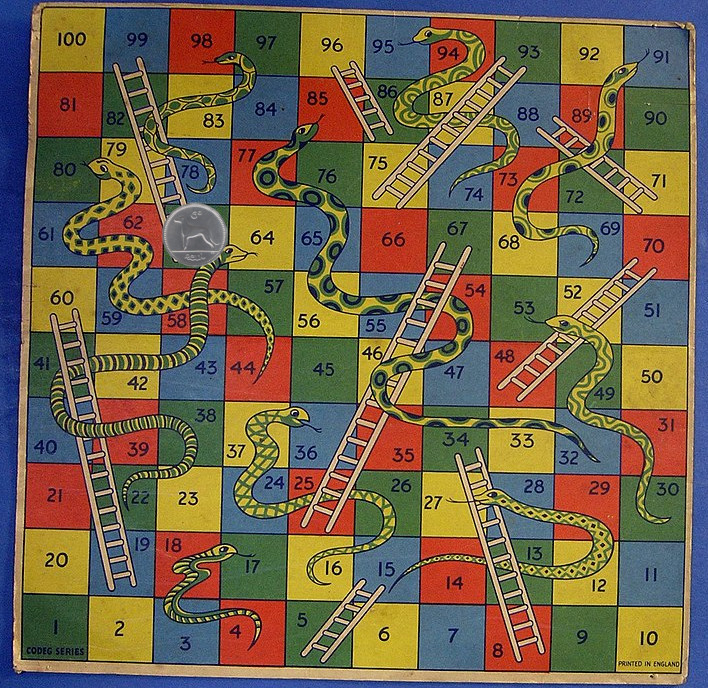
\includegraphics[width=8cm]{game63.jpg}
  \end{center}
    \vfill
\tiny{\flushright{Image from wikipedia.}}
\end{frame}


\begin{frame}{1$\rightarrow$15$\rightarrow$19$\rightarrow$60$\rightarrow$63$\rightarrow$99 (up the ladder)}
  \begin{center}
    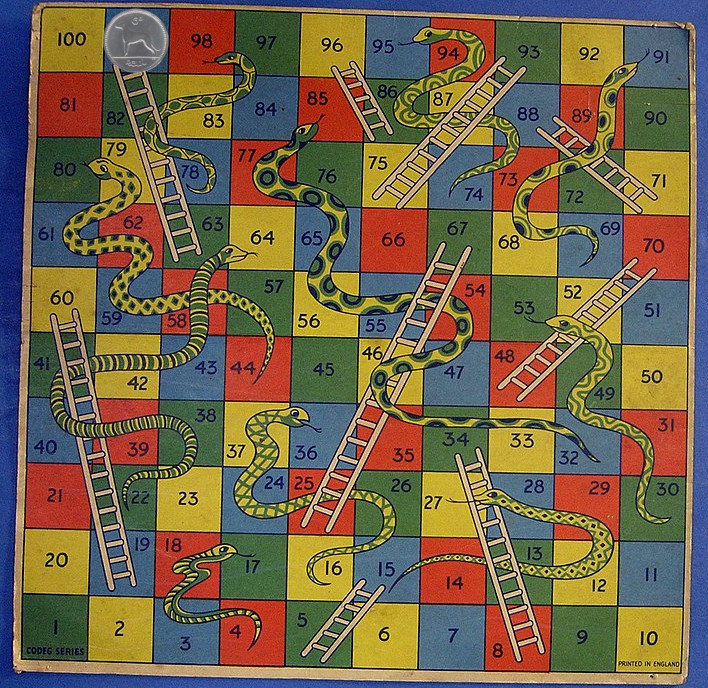
\includegraphics[width=8cm]{game99.jpg}
  \end{center}
    \vfill
\tiny{\flushright{Image from wikipedia.}}
\end{frame}


\begin{frame}{(4,4,3)}
  \begin{center}
    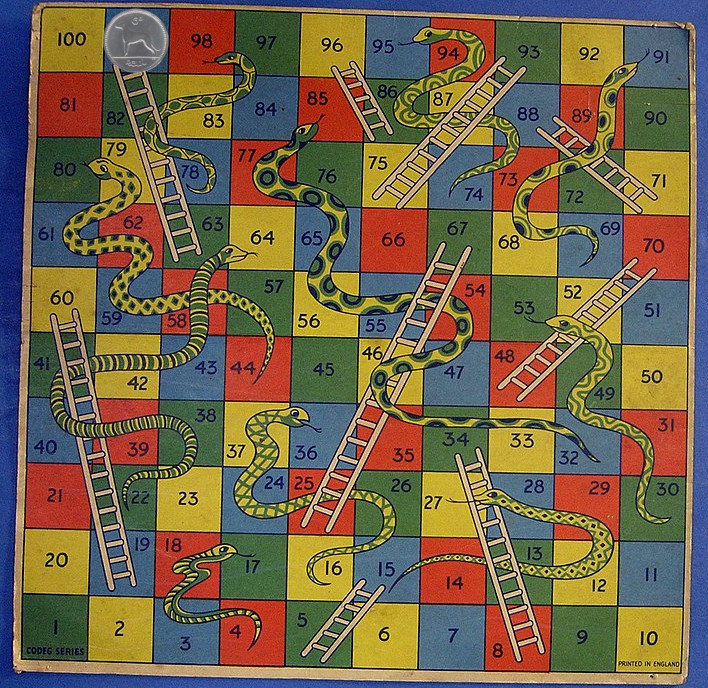
\includegraphics[width=8cm]{game99.jpg}
  \end{center}
    \vfill
\tiny{\flushright{Image from wikipedia.}}
\end{frame}


\end{document}

